\documentclass[12pt]{article}

\usepackage{geometry}
\geometry{letterpaper, portrait, margin=1in}

\usepackage{helvet}
\renewcommand{\familydefault}{\sfdefault}

\usepackage{setspace}
\onehalfspacing

\usepackage{algorithm}

\usepackage{algpseudocode}

\usepackage{graphicx}

\graphicspath{ {img/} }

\title{Predicting motion from LFP data--a comparison between temporal and spectral methods}
\author{Jackson Cornell, Maxwell Rosenzweig}
\date{\today}

\begin{document}

\maketitle


\section{Background and Significance}

Brain-Computer Interfaces (BCIs) are an emerging technology for medical applications such as neural rehabilitation for disabled individuals. BCIs allow for the processing of neural signals to either transduce an action or provide a feedback stimulus to the brain. For our project, we will consider the processing of Local Field Potential (LFP) signals to predict hand and arm movement captured by accelerometer data. We can use this predictive model to translate the thought of movement and resultant LFP into a variety of outcomes such as movement of a prosthetic, control of a cursor on a screen, or interaction in a Virtual Reality (VR) space, among other applications of the produced accelerometer data.

These particular outcomes are significant for a variety of applications: A prosthetic could be developed for individuals who have lost a limb; a cursor control system could help someone who has lost control or limited control of their limbs; commercial applications such VR could be developed.

The aim of our project is to develop a BCI which will predict the desired movement (i.e. accelerometer data) given the corresponding LFP data. We will compare two approaches to decoding LFP data, the first using the spectral power of different frequency bands, and the other using the temporal dynamics. These will be decoded using a Convolutional Neural Network (CNN) and Kernel Least Mean Squares (KLMS) filter, respectively.


\section{Preliminary Studies}

One of the most persistent ongoing debates in computational neuroscience is if neural information is encoded in the frequency domain, the time domain, or a combination of both. One of the most common processing techniques for neural signals is binning the spike train data into a spike train average (STA), which effectively computes the frequency over windows of time. Other methods use adaptive filters such as the Kalman or Wiener filter to encode the time-domain dynamics of the signal to predict an output. In this paper, we compare the performance of two separate models, the CNN and the KLMS, which will decode the LFP signals from their frequency and time domain representations, respectively.

Convolutional neural networks have gained considerable attention in recent years with many applications ranging from natural language processing to medical image analysis and image classification. Essentially, CNNs are multi-layer neural networks composed of several convolution-pooling layers followed by nonlinear activation units and fully connected layers.
These layers are stacked such that the input data is passed through all connected layers to drive the output of the network. 
 \cite{krizhevsky2017}

Wiener filters are a widely used algorithm for estimating the dynamics of a system and predicting the outcome given some input. In practice, however, the Wiener filter falls short of expectations. The first reason being its assumption that the system it is modeling is wide sense stationary (WSS), and the second being its matrix inversion having a complexity of $O(n^3)$. For an algorithm expected to run on a resource-constrained BCI, both of these facets make it impractical to deploy. Luckily, 70 years of signal processing research has found many ways to circumvent these issues. \cite{li2012}

Instead of doing a matrix inversion to find the optimal model parameters, these parameters can instead be found using stochastic gradient descent (SGD). SGD basically computes the MSE between the estimated signal and the actual signal, and uses this error to descend down the learning manifold to the optimal parameter values. Given the same assumptions the Wiener filter makes about the signal being WSS, the SGD approach is guaranteed to find the optimal parameters with $O(n)$ complexity. This approach is known as the Least Means Squares (LMS) filter. \cite{li2012}

The next problem to solve is the fact that LFP data is not WSS. Kernel methods are known to be able to handle cases such as these. Kernel methods map the input data into a higher-dimension feature space where optimal weights can be found. This allows non-Gaussian and non-linear system’s dynamics to be estimated. The Kernel LMS (KLMS) filter is a kernelized version of LMS filter, and can be used to train data on-line. We will use the KLMS to decode the time-domain LFP signal into accelerometer data. \cite{li2012}


\section{Research Design and Methods}

\subsection{Dataset}

Our dataset comes from Oweiss Lab patient data. At the lab, patients are undergoing treatment for tremors using deep brain stimulation (DBS). Patients were instructed to do a variety of tasks, such as draw a spiral or move an object to a specified location. These tasks were repeated over a number of sessions. During each task, custom software called alpine recorded their movement with an accelerometer, an EMG using electrodes, and LFP data using an implant. 

For the purposes of our study, we are only concerned with the resulting movement from neural activity. As such, we will be ignoring the splits of tasks in each session and the metadata for sessions (i.e, task type, date, other metadata). However, it is important that we process each session separately, as sensor placement and configuration may vary slightly between sessions.

We will split the dataset into a training and test dataset. Following the standard for constructing machine learning models, this will consist of 80\% for training and 20\% for testing. The testing set will be further split into several folds for cross-validation of optimal hyperparameters (this process will be repeated for each model).

First, we will split the dataset as described above. 80\% of the sessions will make up the training set, and the remaining 20\% will make up the testing set. The session identifiers will be stored in tables. We will use the provided "read\_data.m" program to import the data into a readable ".mat" file, and will feed the program the data from our tables to get the session data for further processing.

\subsection{Data Pre-Processing}

To increase model performance, we will employ bandpass filtering and downsampling of the accelerometer data. The data will be preprocessed in a manner in which different features will be extracted for inputing into the KLMS and CNN models.

The LFP raw channel data, which are differential signals, will be subtracted from one another to get 2 de-noised signals. Studies show that the gamma band of LFP signals have a strong correlation with reach goals \cite{hwang2012}. Thus, the LFP data will be bandpass filtered from 30-80 Hz, which will act as the input to the KLMS model. For kernel-based methods, the trajectory can be decoded directly from the time domain signal \cite{li2012}. The spectrograms for the CNN model, on the other hand, will be computed directly from the de-noised signals. It is expected that the neural network will learn which frequencies encode the accelerometer dynamics. The spectrograms will be computed with windows of 400 ms, applied every 200 ms \cite{zhang2013}.

\begin{figure}[h]
\caption{Spectrogram of LFP channel}
\centering
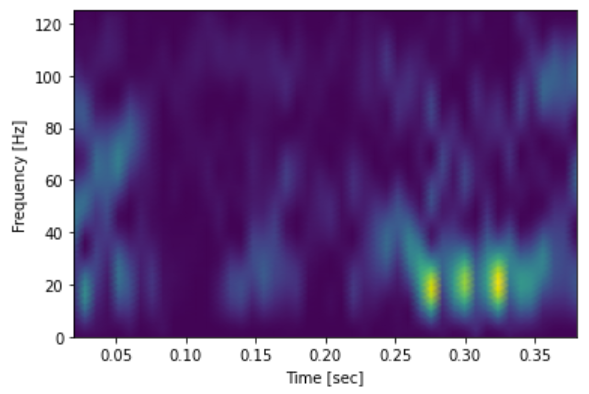
\includegraphics[width=0.5\textwidth]{lfp_spect}
\end{figure}

For the KLMS model, the accelerometer data will be lowpass filtered with a cutoff of 2.5 Hz. This cutoff was decided from data analysis showing there being little to no frequencies present above this range. It was then downsampled to 250 Hz to match the sampling frequency of the LFP data for ease of model training. To align with the CNN model's spectrograms, the accelerometer data will then be downsampled to a sampling frequency of 5 Hz.

\begin{figure}[h]
\caption{Downsampled accelerometer time series}
\centering
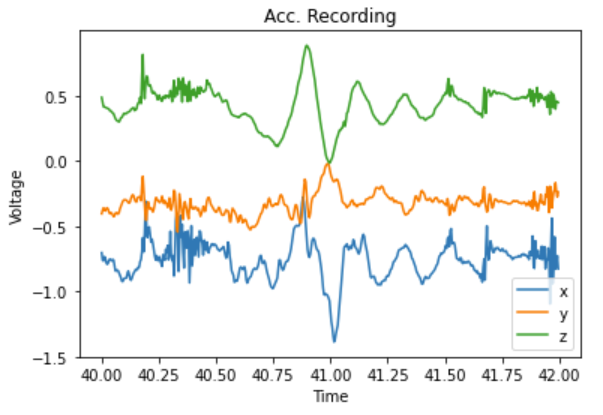
\includegraphics[width=0.5\textwidth]{acc_time_series}
\end{figure}

\subsection{Neural Decoding}

\subsubsection{Kernel Least Mean Squares Filter (KLMS)}

There are few hyperparameters needed to run the KLMS. The first is the filter order, which can be derived from where the autocorrelation function (ACF) of the input data crosses zero. The other two are the kernel width and step size, which will each be found by using hyperparameter tuning described above. Below presents the algorithm for computing the KLMS, given these hyperparameters:

\begin{algorithm}
\caption{KLMS}\label{alg:cap}
\begin{algorithmic}
   \Require step size $\mu$, filter order $M$, and kernel size
   $\sigma$ initialized  
   \State $k(x_i, x_j) = exp(-|| x_i - x_j ||^2_2 / \sigma^2_x)$
   \State $a^{(0)} \gets 0$  
   \For{each vector of size $M$ in $x_n$}  
     \State $f_i \gets \sum_{n=1}^{N} a^{(i)} k(x_i, x_n)$\   
     \State $e_i \gets y_i - f_i$    
     \State $a^{(i+1)} \gets a^{(i)} + \mu e_i$   
   \EndFor 
\end{algorithmic}
\end{algorithm}

The KLMS filter will be further modified in the following ways: using vector quantization and an entropy-based learning function for outlier rejection. Vector quantization works in a manner in which, instead of adding a new weight for every incoming sample, if an error calculated from the sample is below a threshold $\epsilon$, an existing weight is updated, rather than a new weight added. Along with mean square error (MSE) being used as a criterion for learning, maximum correlation criterion (MCC) will also be used, as it takes into account higher order statistics aand can therefor be used to reject outliers.

\subsection{Convolutional Neural Network (CNN)}

For this regression task, we will design a CNN in Python using the deep learning libraries TensorFlow and Keras. The CNN will consist of multiple convolution layers to create output feature maps. \cite{Angrick2019}

The model layers will consist of a spatial convolution layer, a non-linear activation function, batch normalization and max pooling layers to generate the feature maps. These feature maps will be flattened and passed through fully connected layers, dropout layers and a non-linear activation function to obtain the predicted accelerometer output values. The kernel size, stride, dropout rate, number of hidden layers and more will be initially defined but modified using Hyperparameter training.

\subsubsection{Hyperparameter Tuning}

CNNs need several hyperparameters to construct its architecture, some of which will be found using hyperparameter tuning, others will be found using knowledge of the data. Specifically, since we are essentially performing regression rather than classification of the data, we will use a linear activation function on the output. For the hidden layers, leaky ReLU is known to perform well for CNNs. Hyperparameter tuning will need to be carried out to determine quantities such as kernel size, dropout rate, number of hidden layers, batch size, learning rate, and more. Luckily, python libraries such as Sklearn and Tensorflow have many methods that allow easy tuning of such parameters.

\subsubsection{Training} 

The tensor dataset obtained after preprocessing the raw LFP data will be of the shape $N$x$C$x$H$x$W$, where $N$ is the number of Spectrograms, $C$ is the number of channels(i.e., $1$ for the spectrogram data), $H$ and $W$ are the height and width of the image. The dataset will be split following a traditional 80/20 split for ML models, where 80\% of the data is for training the model and 20\% of the data is for validating the model.

The input to the CNN will be an input tensor of the Spectrogram of LFPs in batches, each individual spectrogram can be considered as a single channel image over a window of time. The output of the data generated will be a three-dimensional vector corresponding to the three axes of acceleration $(x, y, z)$.

The weights and biases of the CNN are calculated using a back-propagation algorithm, where the labeled training set is exposed to the network and the error $e$ between the desired output and the predicted output by the network is calculated \cite{hecht1992}. The loss function used to calculate the error will be the Mean Squared Error (MSE) function and the Adam optimization algorithm will be used to modify the training weights. The optimal number of epochs and the learning rate for training the network will be defined using hyperparameter tuning.

\subsection{Performance Analysis}

The predicted accelerometer data will be compared to the actual accelerometer data to produce an error measurement, which will be used to assess their performance as well as calculate the model parameters. Once model training is complete, the models will be evaluated using the test set. Other metrics that will be considered are the computational cost (how long it takes each model to process an input) and memory usage (how much memory does the model use to process an input). With these metrics, we will be able to compare the performance and accuracy of these different models, and--more specifically--which ones will be best suited for use in a BCI.

We will use a least squares error to compare the predicted accelerometer data to the session data from the test set. Because the predicted data and session data will have different sampling frequencies, we will compare the downsampled session accelerometer data to the predicted accelerometer data. We can then graph this error over time to compare the models, as well as compute the average error and variance of the error for the models to compare accuracy and precision as well.

For computational cost, we will time the models on each test session and compare the average runtime. Similarly, we will measure and compare average memory usage.


\section{Results}

\subsection{KLMS}

The KLMS was traied on 300 seconds of LFP data. Model test evaluation showed the KLMS could not effectively encode the accelerometer trajectory. The model is able to encapsulate the training data near perfectly, but severely underperforms with the testing data, indicating overfitting. The below table shows what hyperparameter values were tested:

\begin{center}
\begin{tabular}{ |c|c| } 
\hline
Hyperparameters & Values\\ 
\hline
Kernel size $\sigma_x$ & 0.1 \\ 
Embedding size $k$ & 40\\
Step size $\eta$ & 0.5\\
Threshold $\epsilon$ & 0.05\\
Criterion & MSE, MCC\\
Entropy kernel size $\sigma_h$ & 1\\
\hline
\end{tabular}
\end{center}

The below plots show the model training results on the hyperparameters with a minimum MSE:

The reasons for the KLMS overfitting the data are numerous. One possible explanation is that in this instance, the gamma band does not infact encode reach goals. In this case, there is no correlation between the input bandpass filtered LFP data and the output accelerometer trajectories. Additionally, an insufficient grid search of hyperparmeters may have been performed, in which case the model parameters would be sub-optimal. Finally, it is possible that the temporal dynamics of LFP signals do not, in fact, carry enformation for cognitive motor control.

\subsection{CNN}


\section{Discussion}


\bibliography{report}
\bibliographystyle{ieeetr}

\end{document}